This section is meant to describe the performance-relevant implementation details. First, the \textsc{Dataset} module is described as the join described in section \ref{section_executing_the_join} needs to be performed efficiently using the heuristics proposed. Next, the building process of the grouping function $\Gamma_\text{nodes}$ corresponding to the set $R_{d,u}$ from section \ref{section_tree_based_models} is found, while also describing the structure of the \textsc{ShadowModels} module. Subsequently, the role of caching and lazy calculation of results is outlined. Finally, approaches to parallel computing using the visualization algorithm are touched upon.

\subsection{The Dataset Module}
As shown in Figure \ref{fig:implementation_dataset}, the module contains three classes: the \emph{Dataset}, the \emph{BaseDataset}, and the \emph{ProcessedDataset} class. All of them make extensive use of the pandas data frame, which allows storing two-dimensional tabular data with the capability to index the rows by a column. In this work, the index column in a data frame will be unique and, therefore, the data frame index implies a functional dependency, analog to a key in a relation of a relational database.

\begin{figure}
    \centering
    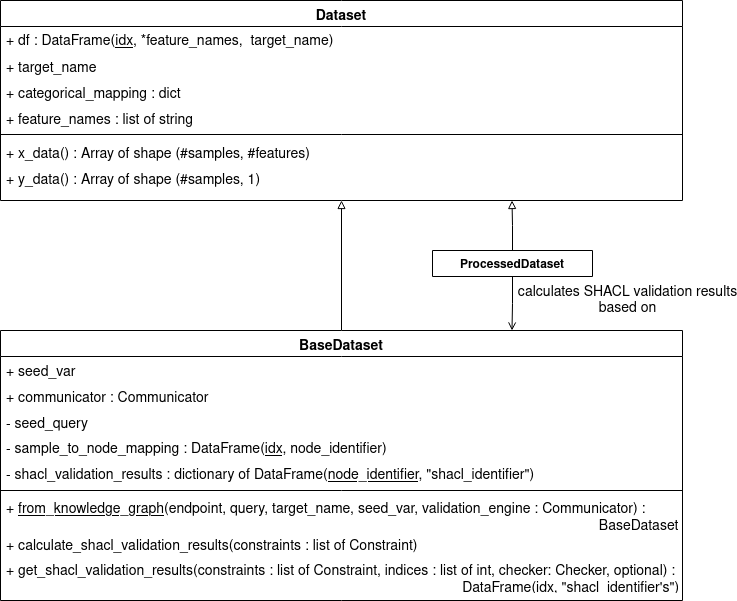
\includegraphics[width=0.8\textwidth]{images/implementation/class_diagram_dataset.png}
    \caption{The \textsc{Dataset} Module}
    \label{fig:implementation_dataset}
\end{figure}

The \emph{Dataset} class is a generic class holding the whole dataset in a pandas data frame called ``df'' with an index column idx, a column for each feature, and a column for the target. In analogy to a relation in a relational database, the type of the data frame will be denoted by \emph{DataFrame}(\underline{idx}, *feature\_names, target\_name)\footnote{* here denotes the unpacking of the followed list}.
Therefore, the feature names and the target name need to be stored to identify the problem instances (the ``x\_data'') and the target (the ``y\_data''). A dictionary called ``categorical\_mapping'' is used to give the user the option to map each feature to a dictionary, which maps encoded feature values to meaningful terms. For example, in a classification task with a \emph{Dataset} containing encoded target classes ``categorical\_mapping[target\_name]'' is a dictionary mapping the encoded target classes to their decoded class names.

The \emph{BaseDataset} extends the \emph{Dataset}, with the notion of the samples-to-node mapping, which is realized by a \emph{DataFrame}(\underline{idx}, node\_identifier). Each entry in the data frame maps an index $i$ of a sample in the dataset to the node $\eta(i)$. At this point, it should be mentioned that \emph{DataFrame}(\underline{idx}, *feature\_names, target\_name) and \emph{DataFrame}(\underline{idx}, node\_identifier) can be concatenated to give the $T$ relation mentioned in section \ref{section_executing_the_join}. The concatenation does not require a join as both are only stored separate for implementation convenience.

The \emph{BaseDataset} is assumed to be retrieved from a knowledge graph with a user defined query from a given endpoint using the underlined static method of the same name. In contrast to definition \ref{Def:transforming_tuple_to_dataset}, the user is allowed to specify the seed variable and the target variable (target\_name) to be different from ?x and ?t. A SHACL validation engine communicator is needed, which provides a method to perform the SHACL validation given a set of constraints. The \emph{BaseDataset} starts the SHACL validation process and stores its results in a dictionary ``shacl\_validation\_results'' mapping (shape schema, target shape) tuples (here called ``shacl\_identifier'') to \emph{DataFrame}(\underline{node\_identifier}, shacl\_identifier). Each entry assigns a SHACL validation result to a node in the knowledge graph. The construct thereby represents the \textit{validate} function in algorithms \ref{algo:validation_engine} and \ref{algo:reduced_shacl_validation}. The SHACL validation is triggered by calling ``calculate\_shacl\_validation\_results''. Each data frame in ``shacl\_validation\_results'' corresponds to a relation $S_{j,k}$ in section \ref{section_executing_the_join}.

However, during the constraint evaluation, the SHACL validation results are needed per sample. Therefore, the method ``get\_shacl\_validation\_results'' produces SHACL validation results joined as described in section \ref{section_executing_the_join}. Implementation-wise, the procedure results in a \emph{DataFrame}(\underline{idx},"shacl\_identifier's") mapping each index of a sample to SHACL validation results. The implementation makes use of the join method provided by the pandas library and attempts to make use of the join heuristics from section \ref{section_executing_the_join}. First, the heuristic from lemma \ref{S:join_heuristic1} is implemented in a greedy manner: The SHACL validation results per constraint are grouped by their target definition and ordered according to their average size. Joining in the order estimated should keep the number of different entities with SHACL validation results in the intermediate results small, such that the size of intermediate results increases gradually.
Secondly, the heuristic from lemma \ref{S:join_heuristic2} is implemented by joining the SHACL validation results first by default, as there is no need for intermediate SHACL validation results in the current implementation.

\begin{figure}
    \centering
    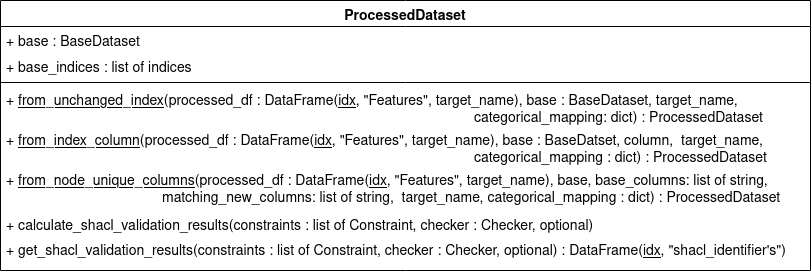
\includegraphics[width=0.8\textwidth]{images/implementation/class_diagram_processed_dataset.png}
    \caption{The \emph{ProcessedDataset} Class}
    \label{fig:implementation_processed_dataset}
\end{figure}

\begin{figure}
    \centering
    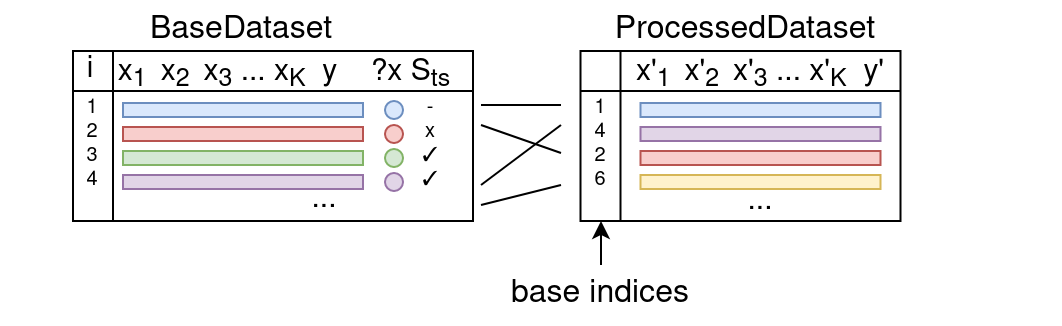
\includegraphics[width=0.8\textwidth]{images/implementation/base_indicies.png}
    \caption{\textbf{Reconstructing the Sample-to-node Mapping of a Modified Dataset:} The left-hand side shows the \emph{BaseDataset} extracted from the knowledge graph with the seed nodes ?x and the SHACL validation results $S_{ts}$. The right-hand side shows a processed version of the dataset called \emph{ProcessedDataset} with reconstructed base indices such that the results associated with the original \emph{Dataset} can be used}
    \label{fig:base_indices_viz}
\end{figure}

The last class is the \emph{ProcessedDataset} (as depicted in Figure \ref{fig:implementation_processed_dataset}), which allows the user of a \emph{BaseDataset} to modify the data frame ``df'' (the original dataset) as needed. In contrast to the pseudocode provided in algorithm \ref{algo:validation_engine}, one cannot expect that the original dataset extracted from the knowledge graph is the final dataset, which can be used to train, validate or test the model (see example \ref{Bsp:applying_the_validation_engine}). However, the sample-to-node mapping that was originally extracted when the \emph{BaseDataset} was created must remain intact when the original dataset is modified. 

This is effectively tackled by a mapping called ``base\_indices'' from the new indices $i$ to the old ones $j$ in the \emph{BaseDataset} (see Figure \ref{fig:base_indices_viz}). The mapping is represented as a list in which the $i$-th element contains the corresponding index $j$. The static methods are provided for the user to create the \emph{ProcessedDataset} depending on the changes done to the original dataset, represented as \emph{BaseDataset}. In the best case, the index column of the original dataset was kept or copied to a new column before the modifications were done. As modifications like dropping or duplicating samples will now affect the original index column, the mapping can be read from the index or copied column respectively. If that is not the case, the final dataset has to be joined with the original dataset on a column with values unique to the original index values.
In both cases, the result is a \emph{ProcessedDataset}, representing the final dataset, in which every sample can be mapped to the original seed node and the SHACL validation results associated with them.

\subsection{Estimating the Decision-tree-node-to-samples Mapping}
\label{section_decision_tree_node_to_samples_mapping}
After the validation engine is done and the constraint validation results are available, the validation results are summarized with respect to the model provided. In the case of decision trees, a decision-tree-node-to-samples mapping is needed. That is, the assignment made in section \ref{section_tree_based_models} by the set $R_{d,u}$ for each node $n_{d,u}$ in the decision tree or the grouping function $\Gamma_\text{nodes}$ from section \ref{section_constraint_decision_tree_visualization}. This is very relevant to performance, since the number of nodes in the decision tree increases exponentially with the depth of the decision tree.

\begin{figure}
    \centering
    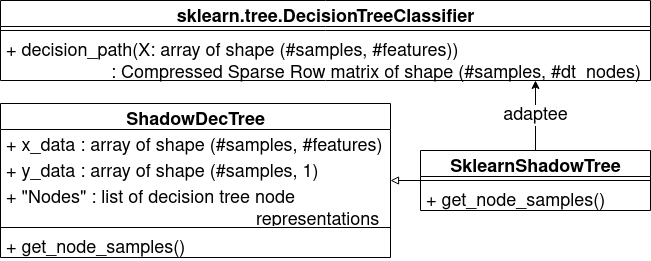
\includegraphics[width=0.6\textwidth]{images/implementation/ShadowModelAdapterPattern.png}
    \caption{Usage of the Adapter Pattern in the ShadowModels Module (see \cite{dtreeviz})}
    \label{fig:adapterPatternShadowModels}
\end{figure}

Implementation-wise, each node in the decision tree has a unique identifier and the goal is to retrieve a dictionary mapping each identifier to a list containing the indices in the dataset associated with the samples handled by that node. 

To further understand the implementation, Figure \ref{fig:adapterPatternShadowModels} shows the structure of the \textsc{ShadowModels} module. In general, the module is responsible for providing insights into the trained model needed for the visualizations. As this should be independent of the library used to train the model, the adapter pattern is used. The \emph{ShadowDecTree} class provides the interface for the library-agnostic adapter. Multiple adapters are already implemented in the dtreeviz library \cite{dtreeviz}. As an example, Figure \ref{fig:adapterPatternShadowModels} shows the adapter class \emph{SklearnShadowTree} which implements the \glqq get\_node\_samples\grqq{} method using the \glqq decision\_path\grqq{} method from a given an instance of a trained \emph{DecisionTreeClassifier} of the scikit-learn library. 

\begin{figure}
    \centering
    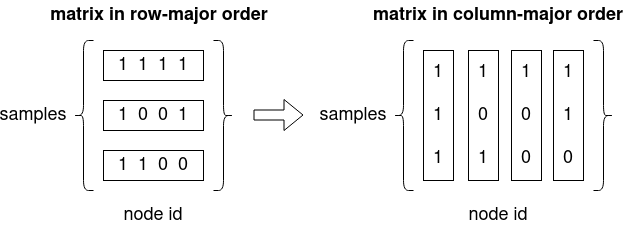
\includegraphics[width=0.6\textwidth]{images/implementation/row-to-column-major-matrix.png}
    \caption{Converting a Row-major Matrix into a Column-major Matrix}
    \label{fig:rowToColumnMajor}
\end{figure}

The ``decision\_path'' method gives a matrix $M \in \{0,1\}^{\textrm{\#samples} \times \textrm{\#decision\_tree\_nodes}}$ with a nonzero entry at position ($i$,$j$) indicating that the sample $i$ is handled by the node $j$. As it is typical for Python, the matrix is saved in row-major order. That means, the rows of the matrix are physically stored next to each other. Therefore, it is recommended for the inner loop to address the column $j$ when iterating over the entries of the matrix in a nested loop. The implementation of the ``get\_node\_samples'' method provided by the dtreeviz library does exactly that while adding $i$ to the list referred to by the decision-tree-node-to-samples mapping with entry $j$ if $M_{i,j}$ it is nonzero. Therefore, accessing the Python dictionary structure and adding an item to Python list $\textrm{\#samples} * \textrm{\#decision\_tree\_nodes}$ times. 

However, as vectorized code execution using NumPy turns out to be faster in many cases \cite{numpy}, the following heuristic is proposed:

\begin{Satz}{Efficiently Estimating the Decision-tree-node-to-samples mapping}{}
    The decision-tree-node-to-samples mapping should be estimated using vectorized code execution.
\end{Satz}

Implementation-wise, $M$ is converted into a column-major form (see Figure \ref{fig:rowToColumnMajor}) and the nonzero row indices of each column $j$ are written into the decision-tree-node-to-samples mapping with entry $j$. This results in accessing the Python dictionary only $\#samples$ times and avoids the usage of the Python lists.

\subsection{Caching and Calculating the Needed Intermediate Results}
During the constraint validation process and the following visualization process, specific intermediate results are needed multiple times. Therefore, the goal is to calculate them only once and cache them if needed.

\paragraph{SHACL Validation Results} When validating multiple constraints that refer to the same SHACL shape schema, sequential validation would lead to the duplicate evaluation of SHACL shapes. To avoid this, the SHACL validation of multiple constraints is performed according to the heuristics described in section \ref{section_shaclapi}. These heuristics further minimize the load on the SHACL engine by simultaneously reducing the SHACL schema to the needed shapes and targets. The heuristics were implemented in an API because they work independently of the SHACL engine implementation. The API is called shaclAPI and is publicly available in GitHub\footnote{\href{https://github.com/JulianLoewe/shaclAPI}{https://github.com/JulianLoewe/shaclAPI}}. 

\begin{figure}
    \centering
    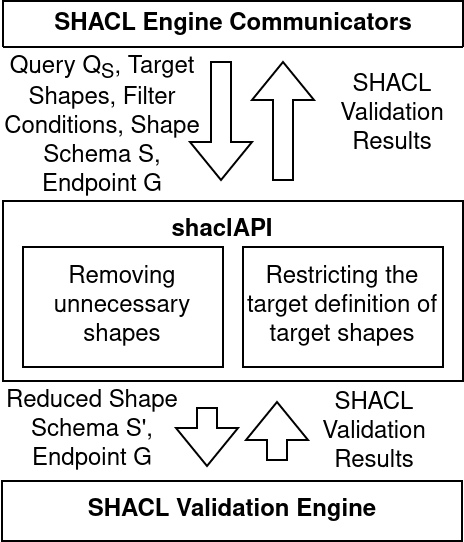
\includegraphics[width=0.4\textwidth]{images/implementation/shacl_api.png}
    \caption{\textbf{shaclAPI:} Reducing Shape Schemas SHACL-engine-agnostically}
    \label{fig:shacl_api}
\end{figure}

Figure \ref{fig:shacl_api} illustrates the process. The \textsc{SHACL Engine Communicators} module contacts the shaclAPI per SHACL schema and set of constraints making use of the schema. Algorithm \ref{algo:reduced_shacl_validation} shows the steps needed. However, the shaclAPI is built purpose-independent and, therefore, needs the seed query $Q_s$ instead of the dataset generating query $Q_D$ (see section \ref{section_propositionalization} for definition and \ref{section_shaclapi} regarding the conversion) for the reduction of the target definitions of the target shapes mentioned in the constraints. In section \ref{section_shaclapi}, the form of prediction constraints is exploited to further reduce the target definitions of the target shapes by pushing filter terms into the target queries of the shapes. These can be provided optionally per target shape and will be squashed together with the original target definition and the given query $Q_S$ into new target definitions. After removing unnecessary shapes and restricting the target definition, when possible, as summarized above and shown in algorithm \ref{algo:reduced_shacl_validation}, the reduced shape schema is forwarded to the SHACL validation engine. The SHACL validation results are returned entity-wise\footnote{That is, separately for each node addressed by the target definitions of the shapes in the shape schema} and incrementally to the user of the shaclAPI. 

The SHACL validation process is originally triggered by the \textsc{Dataset} module, which stores and joins them according to the join strategy (see section \ref{section_executing_the_join}). The raw validation results are stored in the ``shacl\_validation\_results'' dictionary and when joined the ``sample\_to\_node\_mapping'' data frame is extended to additionally store the joined results. The \textsc{Dataset} module also takes care of identifying already validated SHACL schemas in new constraints by calculating MD5 checksums given the serialized representation of the SHACL schema. Therefore, identifying the subset of SHACL schemas given by the constraints.

Storing the results in the \textsc{Dataset} agnostic of the machine learning model allows using the SHACL validation results for multiple machine learning models and training iterations without the need for re-validating the SHACL schemas over the knowledge graph. Further, the given implementation of the \emph{PreprocessedDataset} does not push further \uri{FILTER} terms based on the samples used, but just forwards the need for SHACL validation results to the \emph{BaseDataset} instance. This enables the user of a \emph{BaseDataset} \texttt{base} to create multiple instances of the ProcessedDataset given \texttt{base} without triggering redundant SHACL validations.

\begin{figure}
    \centering
    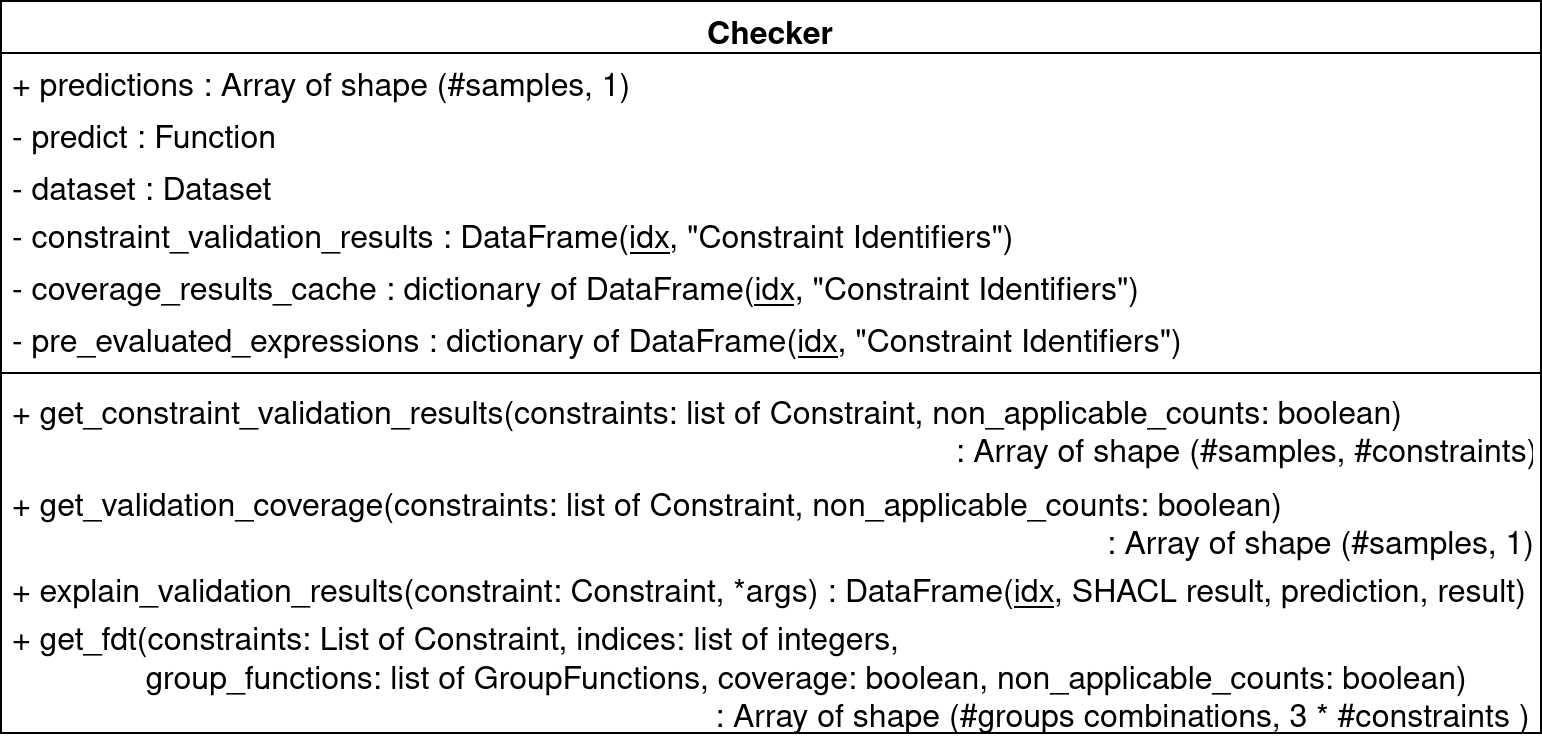
\includegraphics[width=0.8\textwidth]{images/implementation/checker.png}
    \caption{\textbf{The Checker Class}: The \emph{Checker} stores prediction, constraint validation, coverage results and evaluated expression results, and is able to return summarized validation results.}
    \label{fig:checker_implementation}
\end{figure}

\paragraph{Constraint Validation Results and Model Predictions} The \textsc{Checker} module triggers the validation of the constraints over a given machine learning model. An implementation of a class contained in the \textsc{Checker} module is depicted in Figure \ref{fig:checker_implementation}. A checker instance is initialized given a dataset and a predict function representing the machine learning model. Both cannot be changed after initialization, as the checker heavily relies on caching to minimize computation time. Here we assume prediction constraints, as data constraints can be evaluated given only the dataset. A prediction constraint requires, for the evaluation, the predictions of the machine learning model over the problem instances in the dataset. As making predictions can be costly, they are cached (in the ``predictions'' field) to be reused, when evaluating multiple constraints. There are various methods provided by the checker instance, yielding constraint validation results in different formats (see Figure \ref{fig:checker_implementation}). All of them start with requesting the SHACL validation results from the \textsc{Dataset}, calculate the constraint validation results per sample in the dataset, and provide a ``non\_applicable\_counts'' parameter, which let the user choose to use the 3-valued logic or not. Further, the SHACL validation can be interleaved with the constraint validation by evaluating the right-hand side expression of the prediction constraint first, to determine nodes in the knowledge graph, that do not require SHACL validation results (see section \ref{section_shaclapi}). The evaluation results of the right-hand side of the constraints are then stored in the ``pre\_evaluated\_expressions'' field to avoid the recomputation during the final evaluation of the constraint when the needed SHACL validation results are available.

As the validation results are needed in every method and in the case of the decision tree visualization for every node, the results are cached in the ``constraint\_validation\_results'' field.
The model-coherent visualizations (see section \ref{section_constraint_based_explanations}) are based on frequency distribution tables. These can be calculated with the ``get\_fdt'' method. The method unifies the frequency distribution table creation from definitions \ref{Def:frequency_distribution_creation_function} and \ref{Def:coverage}. The latter one is applied if the ``coverage'' parameter is set to true. In that case, the ``get\_validation\_coverage'' method is used to assign each sample in the dataset the constraint validation result with the highest priority (see example \ref{Bsp:coverage_example}). The calculation involves combining multiple validation results, which is why the amount of data needed can make the operation costly, and the results are therefore cached in the \glqq coverage\_results\_cache\grqq{} field. The further parameters of the function correspond to the definitions provided and are generalized to multiple grouping function by formula \ref{multiple_grouping_functions_to_one}.
Finally, the \emph{Checker} class provides a method to explain the constraint validation results by providing the user for each sample in the dataset with the SHACL validation result, the prediction made by the model, and the resulting constraint validation result.

\subsection{Using Parallel Computation for the Visualization Process}
\label{section_parallel_computation}
This section is specific to the decision tree visualization (see section \ref{section_constraint_decision_tree_visualization}) and the algorithm used to compose the different node visualizations. The algorithm is based on the dtreeviz library \cite{dtreeviz} and is by default a sequential process (as shown in algorithm \ref{algo:tree_visualization_algorithm}) with similar options for customization as the dtreeviz library provides. 

\begin{algorithm}[H]
     \caption{Pseudocode of the Constraint Validation Results Annotated Decision Tree Visualization Algorithm}\label{algo:tree_visualization_algorithm}
     \begin{algorithmic}[1]
          \Function{dtreeviz}{Decision Tree $M_\theta$, Constraints $\mathcal{C}$, Checker $H$, boolean \textit{non\_applicable\_counts}, boolean \textit{coverage}, leaf grouping function $\Gamma$}
             \State $\textit{fdts} \gets \emptyset$
             \State $\textit{visualizations} \gets \emptyset$
             \State $\Gamma_\text{nodes} \gets \textbf{getDecisionTreeNodeToSamplesMapping}(M_\theta)$
             \ForEach{$\textit{node} \in \textbf{splitnodes}(M_\theta)$} \label{algo:tree_visualization_algorithm:summary_start}
                \State $f_k \gets \textbf{splitFeature}(node)$
                \State $\textit{fdts} \gets \textit{fdts} ~+~  \{H.\textbf{get\_fdt}(\mathcal{C}, \Gamma_\text{nodes}(\textit{node}), \Gamma_\text{bins}^{f_k}, \textit{coverage}, \textit{non\_applicable\_counts})\}$
             \EndFor
             \ForEach{$\textit{leaf} \in \textbf{leafnodes}(M_\theta)$}
                \State $\textit{fdts} \gets \textit{fdts} ~+~  \{H.\textbf{get\_fdt}(\mathcal{C}, \Gamma_\text{nodes}(\textit{leaf}), \Gamma, \textit{coverage}, \textit{non\_applicable\_counts})\}$
             \EndFor \label{algo:tree_visualization_algorithm:summary_end}
             \ForEach{$\textit{fdt} \in \textit{fdts}$}
                 \State $\textit{visualizations} \gets \textit{visualizations} ~+~  \{\textbf{visualize}(\textit{fdt})\}$ \label{algo:tree_visualization_algorithm:visualize}
             \EndFor
             \State \Return{$\textbf{compose}(\textit{visualizations}, M_\theta)$} \label{algo:tree_visualization_algorithm:compose}
         \EndFunction
     \end{algorithmic}
\end{algorithm}

The algorithm takes as input the constraints $\mathcal{C}$; to be validated over the decision tree $M_\theta$, a checker instance as described in the previous section, two boolean parameters; specifying whether the 3- or 2-valued logic and the coverage from section \ref{section_visualizing_multiple_constraint_validation_results} should be used, and the grouping function, which should be used for the leaves (see section \ref{section_constraint_decision_tree_visualization}). Given the information, the decision-tree-node-to-samples mapping, as discussed in section \ref{section_decision_tree_node_to_samples_mapping}, is calculated and used afterwards to calculate the frequency distribution table of the constraint validation results for each split- and leaf-node according to section \ref{section_constraint_decision_tree_visualization}. 
The frequency distribution tables can then be visualized, as shown in the examples in section \ref{section_constraint_based_explanations}, and need to be composed into the final visualization afterward.

Clearly, the algorithm provides several possibilities for parallel computation:
\begin{enumerate}
    \item[(1)] Validating SHACL schemas over the knowledge graph \label{parallelOption1}
    \item[(2)] Computing the constraint validation results \label{parallelOption2}
    \item[(3)] Summarizing the validation results into frequency distribution tables \label{parallelOption3}
    \item[(4)] Visualizing the frequency distribution tables \label{parallelOption4}
\end{enumerate}

Option (1) would heavily rely on the multiprocessing performance of the SPARQL endpoint or would require multiple instances of the SPARQL endpoint, which is usually not the case. As will become apparent, much of the computational time of the evaluation process (2) is spent on generating the SHACL results (2), and the parallelization of the join would require a library like dask \cite{dask} if one wants to stay with pandas data frame for data management. The implementation of (3) would come either with large main memory requirements or with the need for the validation results to be stored on process-shared read-only memory. 
Currently, the Python implementation supports (4) as this only requires passing the frequency distribution table to the process and allows outsourcing the time needed to create and write the visualizations onto the disk.





%As will be seen in the evaluation chapter, the summary steps (3) and the visualization step (4) of deep decision trees, take long because the number of nodes rise 

%to visualize, which might . %However even (4) comes with a large overhead as process forking is used and therefore all the data cached and stored is copied to each process.